\documentclass[convert={density=1200,size=400x,outext=.png}]{standalone}
\usepackage{pgfplots}
\usetikzlibrary{arrows.meta}
\pgfplotsset{compat=1.11,width=11cm,height=7cm}
\begin{document}
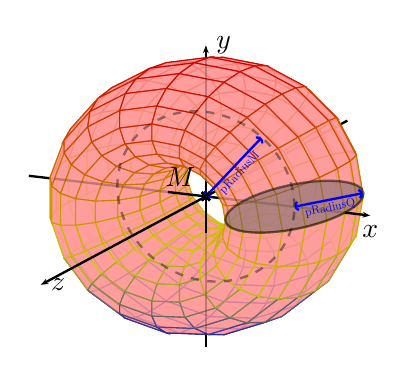
\begin{tikzpicture}
   \begin{axis}[xmin=-1,xmax=3,ymin=-1,ymax=1,zmin=-1,zmax=1,
    axis y line=none,
    axis z line=none,
    axis x line=none,>={Stealth[scale=.4]}, line width=.85pt]
    \draw (-1.4,0,0)--(-.3,0,0) (0,0,0) -- (1.1,0,0);
    \draw[->] (0,0,-1.25)--(0,0,1.25) node[right]{$y$};
    \draw (0,1.2,0)--(0,0,0);
    \addplot3[
      surf,
      fill=red!40,
      fill opacity=.8,
      draw=red!10,
      samples=20,
      domain=0:360,
      y domain=0:360,
      z buffer=sort,
      line width=.4pt
    ]
     ( {(0.7+0.4*cos(x))*cos(y)}, 
       {0.4*sin(x)},
       {(0.7+0.4*cos(x))*sin(y)}
     );
    \draw[->] (0,0,0)--(0,-1.4,0) node[right]{$z$};
    \draw[->] (-.3,0,0)--(0,0,0) (1.1,0,0) -- (1.3,0,0) node[below]{$x$};
    \draw (0,0,-.3)--(0,0,0) node[above left]{$M$};
    \draw[opacity=.2] (-1.2,0,0)--(-.3,0,0) (0,0,0) -- (1.1,0,0);
    \draw[opacity=.2] (0,0,-1.25)--(0,0,1.25);
    \draw[blue,<->, >={Parenthesis[scale=.6]}] (0,0,0) -- node[scale=.3,below,sloped]{\Large pRadiusM} (0.44,0,0.54);
    \filldraw[fill=black!60,opacity=.5,draw=black] (0.7,0,0) circle (.4) plot[mark=x] (0,0,0);
    \draw[draw=blue,<->,>={Parenthesis[scale=.6]}] (0.7,0,0) -- node[blue,scale=.3,below,sloped]{\Large pRadiusQ} (.98, .28, 0);
    %% this crap took me five hours to figure out
    \draw[dashed,opacity=.4] (0.7,0,0)
      \foreach \i in {0,3,...,357} {
        \pgfextra{\pgfmathsetmacro{\A}{0.7*sin(\i)}}
        \pgfextra{\pgfmathsetmacro{\B}{0.7*cos(\i)}}
        -- (\B,0,\A)
      } -- cycle;
  \end{axis}
\end{tikzpicture}
\end{document}
